
\documentclass{beamer}
\usepackage[utf8]{inputenc}
\usepackage{pifont}
\usepackage{caption}
\usetheme{Madrid}
\usecolortheme{default}

\usepackage{algorithm}
\usepackage{algorithmicx}
\usepackage{algpseudocode}
\usepackage{float}

%------------------------------------------------------------
%This block of code defines the information to appear in the
%Title page
\title[Power Analysis Side-channel Attacks] %optional
{Side-channel Metrics}

\subtitle{}

\author[Federico Zanca] % (optional)    
{Federico Zanca}

\institute[] % (optional)
{
  %\inst{1}%
  Computer Science and Engineering\\
  Politecnico di Milano
  %\and
  %\inst{2}%
  %Faculty of Chemistry\\
  %Very Famous University
}

\date[2025] % (optional)
{}

%\logo{\includegraphics[height=1cm]{overleaf-logo}}

%End of title page configuration block
%------------------------------------------------------------



%------------------------------------------------------------
%The next block of commands puts the table of contents at the 
%beginning of each section and highlights the current section:

\AtBeginSection[]
{
  \begin{frame}
    \frametitle{Table of Contents}
    \tableofcontents[currentsection]
  \end{frame}
}
%------------------------------------------------------------


\begin{document}

%The next statement creates the title page.
\frame{\titlepage}


%---------------------------------------------------------
%This block of code is for the table of contents after
%the title page
\begin{frame}
\frametitle{Table of Contents}
\tableofcontents
\end{frame}
%---------------------------------------------------------

\section{Number of Traces}
%---------------------------------------------------------

\begin{frame}
    \frametitle{Number of Traces (N.O.T.): Definition}
    \begin{block}{What it Measures}
        \begin{itemize}
            \item The most commonly used metric to quantify the efficiency of a side-channel attack
            \item It represents the minimum number of side-channel measurements (traces) an attacker needs to successfully recover the secret key
        \end{itemize}
    \end{block}

\newline
    Its primary purpose is to assess how "data-hungry" an attack is. \newline \newline
    A lower N.O.T. indicates a more effective or faster attack, as fewer measurements are required to compromise the secret. \newline \newline
       
        
    
\end{frame}

%---------------------------------------------------------

\begin{frame}
    \frametitle{Number of Traces (N.O.T.): Limitations}
    \begin{block}{Challenges and Limitations}
        \begin{itemize}
            \item \textbf{Attack Dependent:} The N.O.T. value is inherently tied to the specific side-channel attack method employed (e.g., DPA, CPA, Template Attacks), making direct comparisons between different attacks difficult
            \item \textbf{Vague Key Recovery:} The term "key recovery" can be imprecise; it might refer to recovering the full key, a partial key, or simply reducing the entropy of the key space, leading to ambiguity in evaluation
            \item \textbf{Conflates Device and Attacker:} N.O.T. is not an inherent measure of a device's security. It conflates the device's inherent physical leakage with the attacker's computational capabilities (e.g., ability to collect many traces, search the key space). This coalescence makes it difficult to obtain a clear picture of the device's true vulnerability and to identify countermeasures that are robust against any attacker

        \end{itemize}
    \end{block}
\end{frame}
\section{Signal to Noise Ratio}

%---------------------------------------------------------

\begin{frame}
    \frametitle{Signal-to-Noise Ratio (SNR): Introduction and Definition}
    \begin{block}{What is SNR?}
        \begin{itemize}
            \item Standalone metric, it can be obtained directly from side-channel traces without needing to launch a full attack
            \item Provides a quick assessment of the quality of information leakage present in the measurements
        \end{itemize}
    \end{block}

    \begin{block}{}
        \begin{itemize}
            \item SNR quantifies the ratio between the strength of the "signal" $L_d$(the useful, data-dependent part of the leakage) and the strength of the "noise" $L_n$ (the random, useless part) \newline \newline
                    $$L=L_d+L_n=g(V)+L_n$$ \text{        where        } $L_n \sim N (0, \sigma^2 )$.

            \item A higher SNR indicates stronger and clearer leakage, making it potentially easier to exploit
        \end{itemize}
    \end{block}
\end{frame}
\begin{frame}
    \frametitle{Signal-to-Noise Ratio (SNR): Introduction and Definition}
    \begin{block}{Mathematical Definition}
            Formally, SNR is defined as the ratio of the variance of the deterministic leakage to the variance of the noise:
            $$ \text{SNR} = \frac{\text{Var}(L_d)}{\text{Var}(L_n)} $$
    \end{block}
\end{frame}


\begin{frame}
\frametitle{SNR: Understanding and Utilizing Leakage}
    \begin{block}{Interpreting SNR}
        \begin{itemize}
            \item A high SNR indicates that the signal component dominates the noise, suggesting clear leakage points
            \item Helps in identifying the most promising Points of Interest (POIs) within a trace, where the leakage is strongest
            \item Can be used to compare the leakage characteristics of different implementations or countermeasures
        \end{itemize}
    \end{block}
\end{frame}







%---------------------------------------------------------

\begin{frame}
    \frametitle{Computing SNR with Simulated Leakage}
    
            In this scenario, the attacker explicitly simulates the leakage $L$ \newline
            This is done by precisely defining its deterministic part ($L_d$) and its noise component ($L_n$)
   

    \begin{block}{Example: 8-bit Value Leakage}
        \begin{itemize}
            \item Simulate the leakage of an 8-bit value $V$ (uniformly random)
            \item Choose a leakage function $g(V) = \alpha V + \beta$, where $\alpha, \beta$ are known constants
            \item Thus, $L_d = \alpha V + \beta$, representing a scaled and offset version of identity leakage
            \item Choose noise $L_n \sim \mathcal{N}(0, \sigma^2)$, specifying $\sigma^2$
            \item The simulation can be noiseless ($\sigma = 0$) to identify leakage, or noisy ($\sigma \ne 0$) to analyze device/countermeasure behavior in the presence of noise
        \end{itemize}
    \end{block}
\end{frame}


\begin{frame}
    \frametitle{SNR with Simulated Leakage: Computation}
    
            In this controlled simulation, we can proceed to compute the SNR directly using the expectations $E(\cdot)$
       

    \begin{block}{Expectations of Deterministic Leakage}
        \begin{itemize}
            \item Expected value of $L_d$:
            $$ E(L_d) = E(g(V)) = \sum_{v=0}^{255} g(v)Pr(v) = \frac{1}{256} \sum_{v=0}^{255} (\alpha v + \beta) $$
            \item Expected value of $L_d^2$:
            $$ E(L_d^2) = E(g(V)^2) = \frac{1}{256} \sum_{v=0}^{255} (\alpha v + \beta)^2 $$
            \item $$ \text{SNR} = \frac{\text{Var}(L_d)}{\text{Var}(L_n)} = \frac{E(L_d^2) - E(L_d)^2}{\sigma^2} $$

        \end{itemize}
    \end{block}
\end{frame}

\begin{frame}
    \frametitle{SNR with Real Measurements}
    \begin{block}{}
        \begin{itemize}
            \item In a real-world scenario, we cannot directly observe the deterministic leakage ($L_d$) or the noise ($L_n$). We can only measure their sum, the total leakage ($L$).
            \item Our goal is to estimate the SNR from these real measurements without prior knowledge of the leakage function.
        \end{itemize}
    \end{block}
        Let's consider once again an example in which the leakage $L$ of an 8-bit value $V$ is observed, obtaining $n$ traces $l_1, ..., l_n$, each trace $l_i$ containing a single time sample that leaks information about $V$
\end{frame}
\newcommand{\Lagr}{\mathop{\mathcal{L}}}
\begin{frame}
    \begin{block}{Estimation Steps}
        \begin{itemize}
            \item 1. Partition traces: Group traces based on the value of the intermediate V (e.g., 256 groups for an 8-bit value). This way we obtain $\Lagr_0,\Lagr_1,...,\Lagr_{255}$. The set $\Lagr_v$ contains all traces $l$ that are observed when $V=v$
            \item 2. Estimate Means: Compute the mean trace $\hat{\mu}_v$ for each $\Lagr_v$ and the overall mean $\hat{\mu}$ . $$\hat{\mu}_v=\frac{1}{|\Lagr_v|}\sum_{l \in \Lagr_v} l$$ $$\hat{\mu}=\frac{1}{256}\sum_{v=0}^{255}\hat{\mu}_v$$ where $|\Lagr-v|$ is the number of traces for the group
        \end{itemize}
    \end{block}
\end{frame}

\begin{frame}
    \begin{block}{}
        \begin{itemize}
            \item 3. Estimate Variances: Compute the variance ($\hat{\sigma}_v^2$) for each group and the average of these variances ($\sigma^2$) as the noise variance.
            $$\hat{\sigma_v^2} = \frac{1}{|\Lagr_v|-1}\sum_{l \in \Lagr_v} (l-\hat{\mu_v})^2$$
            $$\hat{\sigma}^2=\frac{1}{256}\sum_{v=0}^{255}\hat{\sigma}_v$$
            \item 4. Compute SNR: The signal variance is the variance of the group means, while the noise variance is the average of the group variances. The SNR is their ratio.
                $$
                \text{SNR} = \frac{\text{Var}(L_d)}{\text{Var}(L_n)} = \frac{\sum_{v=0}^{255}(\hat{\mu}_v - \hat{\mu})^2}{\hat{\sigma}^2}
                $$
        \end{itemize}
    \end{block}
\end{frame}



%---------------------------------------------------------

\begin{frame}
    \frametitle{Interpreting an SNR Plot}
    \begin{block}{Example: Unprotected AES S-box}
        \begin{itemize}
            \item An SNR plot over time reveals when and where the most significant leakage occurs in an operation.
            \item High peaks in the plot correspond to specific time samples where the leakage is strongly correlated with the secret key.
            \item For instance, an unprotected AES S-box implementation on a Cortex-M0 microcontroller shows distinct peaks where key-dependent operations are performed, with an SNR of approximately 0.02.
            \item The overall shape of the SNR plot provides an overview of the inherent leakage of the device for a given implementation.
        \end{itemize}
    \end{block}
\end{frame}
\begin{frame}
\frametitle{}
    \begin{figure}
        \centering
        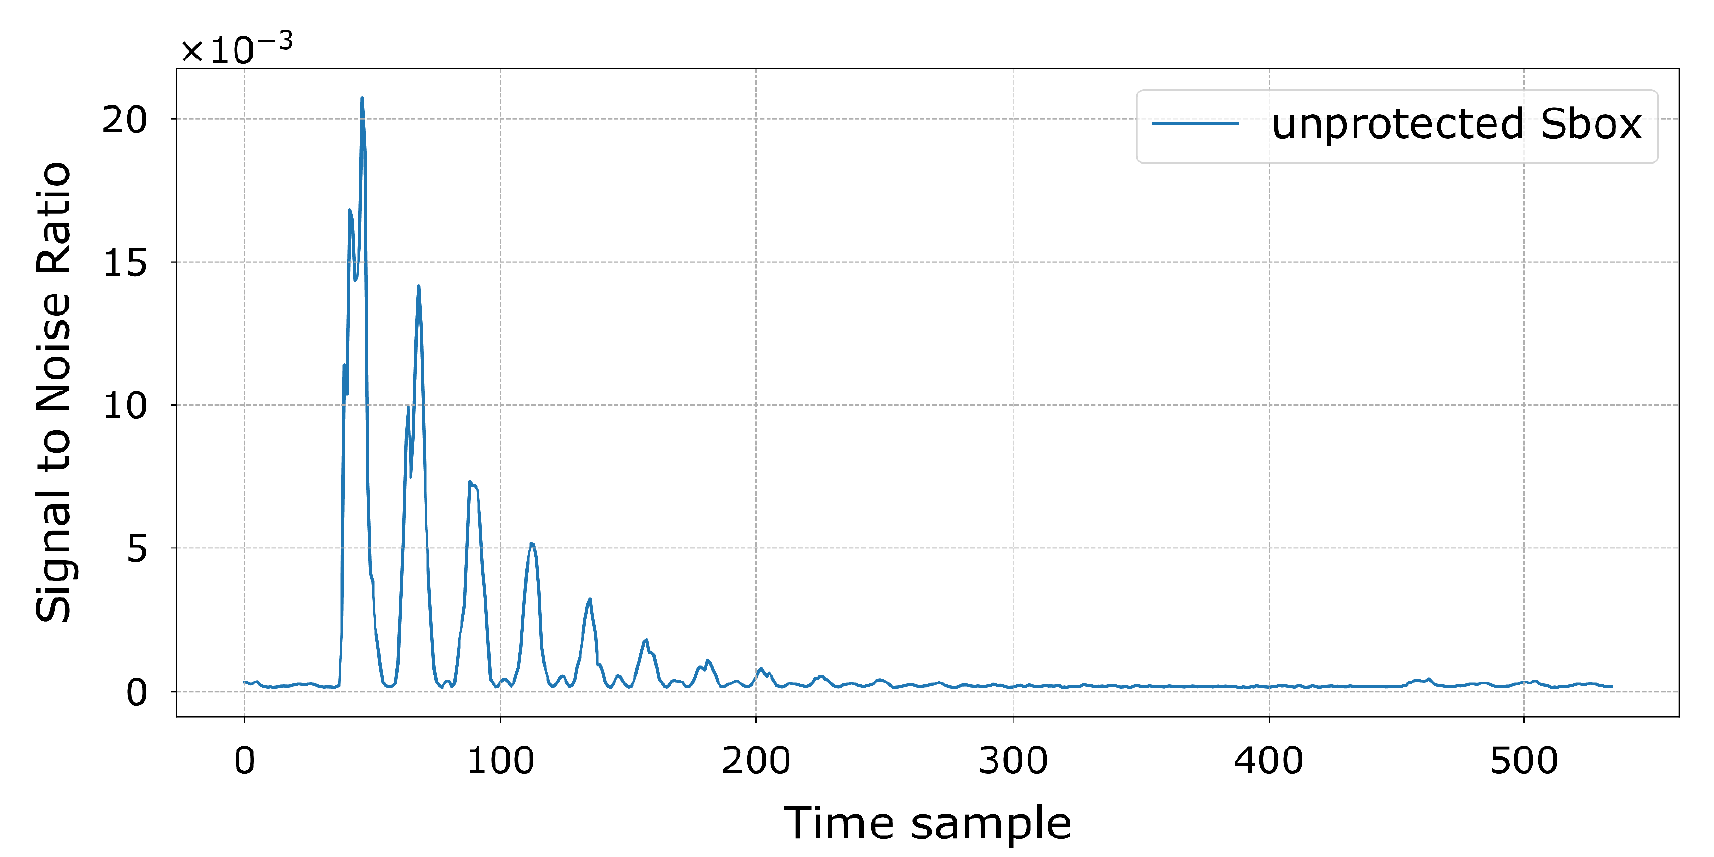
\includegraphics[width=1.0\textwidth]{metrics/Pictures/SNR_plot_unprotected_Sbox.png}
        \caption{SNR plot for an unprotected AES S-box implementation. Peaks indicate key-dependent leakage.}
    \end{figure}
\end{frame}



% Advantages and Limitations
\begin{frame}
    \frametitle{SNR: Limitations}
        \begin{itemize}
            \item \textbf{Not a direct attack feasibility metric:} It maintains a level of generality by not being tied to a specific attack method, but this also means it can't directly convey the actual security level of a device.
            \item \textbf{Simplified leakage model:} The metric implicitly relies on a simplified model of leakage (e.g., assuming a Gaussian noise distribution). In real-world scenarios, the actual leakage may diverge from these assumptions.
            \item \textbf{Parameter estimation issues:} The statistical parameters (mean and variance) must be adequately estimated from the available traces. A poor estimation due to a limited N.O.T. can lead to misleading SNR results.
            \item \textbf{Univariate nature:} The standard definition of SNR focuses on a single time sample at a time (univariate), ignoring the joint multivariate leakage that an adversary can exploit across multiple samples. 
        \end{itemize}
\end{frame}


\section{Score and Rank}

% intro
\begin{frame}
    \frametitle{Score and Rank: Why?}
    The majority of side-channel attacks employ a \textbf{divide-and-conquer} strategy. \newline
       Instead of targeting the full cipher key at once, the attack partitions it into smaller, more manageable parts. For example, a 16-byte (128-bit) AES key is typically attacked as 16 independent key bytes.
    \vspace{1cm}
    \begin{block}{The Goal}
        This approach allows the attacker to recover each small key part individually, dramatically reducing the complexity of the attack. The metrics of \textbf{score and rank} are used to evaluate the success of recovering each of these parts.
    \end{block}
\end{frame}



% Scorie and Rank Process
\begin{frame}
    \frametitle{The Scoring and Ranking Process}
    \framesubtitle{For a Single Key Part (e.g., one AES key byte)}
    For each key portion:
    \begin{enumerate}
        \item \textbf{Hypothesize:} The attacker considers all possible values for the key part. For an 8-bit key byte, this means 256 key candidates (0 to 255).
        \item \textbf{Score:} A score is computed for each key candidate. This score, generated by a distinguisher like correlation, measures how well the hypothesis for that candidate matches the observed side-channel leakage.
        \item \textbf{Guess:} The scores are sorted to produce an ordered list of guesses, from best to worst. The key candidate with the highest score becomes \texttt{guess\textsubscript{1}}, the attacker's top choice. For instance, if candidate k=42 had the best score, then \texttt{guess\textsubscript{1}} would be 42.
        \item \textbf{Rank:} A rank is assigned to each key candidate based on its position in the sorted list. The best-scoring candidate receives rank 1.
    \end{enumerate}
\end{frame}

\begin{frame}
    \frametitle{Algorithm for a Standard Attack with Score and Rank}
    
    \begin{algorithm}[H]
    \begin{algorithmic}[1] 
        \Statex \textbf{Input:} Attack score function $f(\cdot)$, Key candidates $K$
        \Statex \textbf{Data:} Simulated or real side-channel traces
        \Statex \textbf{Output:} $score_k, guess_k, rank_k$, for all $k \in K$ and all key partitions 
        %\Comment{Partition the full cipher key and attack all key parts}
        \State $partitions \gets \text{divide-and-conquer}(\text{full key})$
        \ForAll{$partition \in partitions$}
            %\Comment{Compute the attack score for every key candidate}
            \ForAll{$k \in K$}
                \State $score_k \gets f(\text{traces}, k)$
            \EndFor
            %\Comment{Sort the scores and compute the key guesses}
            \State $[score_i, score_j, \dots, score_m] \gets \text{sort}([score_0, score_1, \dots, score_{|K|-1}])$
            \State $[guess_1, \dots, guess_{|K|}] \gets [i, j, \dots, m]$
            %\Comment{Compute the rank of every key candidate using the key guesses}
            \ForAll{$guess_i$, with $i \in \{1, 2, \dots, |K|\}$}
                \State $rank_{guess_i} \gets i$
            \EndFor
        \EndFor
    \end{algorithmic}
    \end{algorithm}
\end{frame}

\begin{frame}
    \frametitle{Interpreting the Results: Convergence}
    \begin{itemize}
        \item By plotting score/rank against the number of traces, we can visualize the attack's progress.
        \item \textbf{What to look for:} A key candidate that \textbf{stands out} from the rest.
        \item A successful attack shows \textbf{convergent behavior}: one candidate consistently achieves the highest score (and thus, rank 1) as more traces are added.
        \item \textbf{Example:} Considering a CPA attack on AES-128, key candidate $K=203$ reaches rank 1 after about 15,000 traces and maintains that top position, demonstrating a successful recovery of that key byte (as shown in the following pictures). 
    \end{itemize}
\end{frame}

\begin{frame}
    \frametitle{Example: Score and Rank Plot Convergence}
    \begin{figure}
        \centering
        % Score plot
        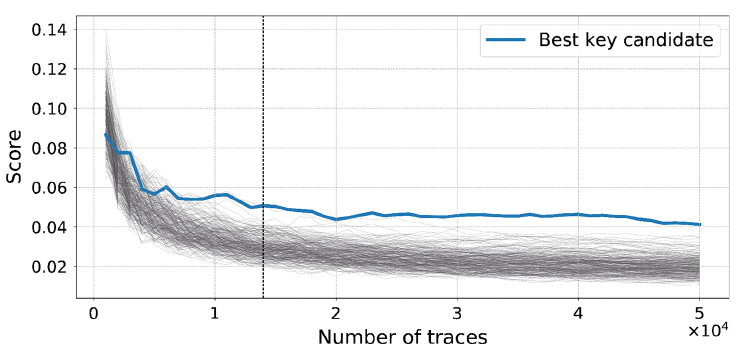
\includegraphics[width=0.55\textwidth]{metrics/Pictures/score_plot.png}
    \end{figure}
    \begin{figure}
        %\vspace{0.5cm} 
        \centering
        % Rank plot 
        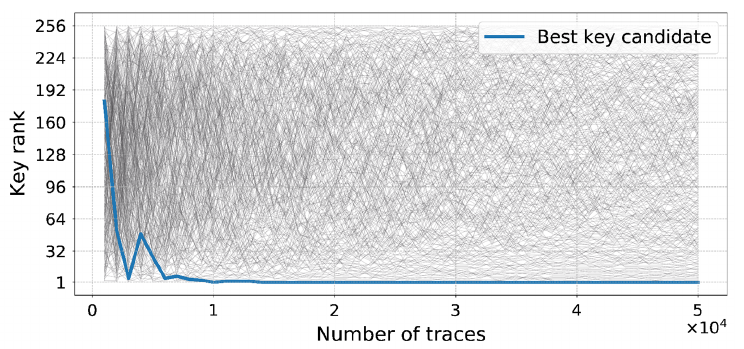
\includegraphics[width=0.55\textwidth]{metrics/Pictures/rank_plot.png}
        \caption{Top: Score plot where the correct key (K=203) is in blue\newline Bottom: Rank plot where the same key's rank converges to 1 after approx. 15,000 traces.}
    \end{figure}
\end{frame}



\begin{frame}
    \frametitle{Limitation: Statistical Stability}

    \begin{block}{The pitfall of a single experiment}
        A score/rank plot is typically generated from one traceset and one fixed key. This can be deceptive. \newline
        A single result might be an \textbf{outlier}, as some keys can be accidentally easier or harder to attack than others.
    \end{block}

        To ensure the results are meaningful, we must follow a more rigorous process:
        \begin{itemize}
            \item \textbf{Repeat} the attack multiple times.
            \item \textbf{Vary} the conditions for each run (e.g., use different keys and different sets of traces).
            \item \textbf{Aggregate} the outcomes by calculating the average score/rank and the standard deviation.
        \end{itemize}
        This gives us a \textbf{statistically stable} metric that truly reflects the device's security.
\end{frame}


\begin{frame}
    \frametitle{Limitation: The Full Key Recovery Problem}

        In a real-world attack, the key is unknown. If the attack is suboptimal or uses too few traces, the correct key parts might not achieve Rank 1. Even if the correct byte is at a low rank (like 2 or 3), the \textbf{device is still vulnerable}, but the full key remains hidden.
    
    
    \begin{block}{Key Enumeration}
        To find the full key, the attacker must perform \textbf{key enumeration}. This is a time-consuming, trial-and-error process:
        \begin{itemize}
            \item Construct full key candidates from combinations of the top-ranking key parts.
            \item Test each full key candidate (e.g., by decrypting a known ciphertext) until the correct one is found.
        \end{itemize}
        This is often a computationally expensive task.
    \end{block}
\end{frame}


\begin{frame}
    \frametitle{The Evaluator's Solution: Known-Key Analysis}

    \begin{block}{A More Efficient Approach for Evaluation}
        To assess security without the high cost of key enumeration, evaluators use a different strategy: a \textbf{known-key analysis}.
    \end{block}
    
    \begin{itemize}
        \item In this scenario, the evaluator knows the secret key from the start.
        \item This allows them to check the rank of the \textit{correct key} directly, even if the attack fails to place it at Rank 1.
        \item This answers the question "How close are we to breaking it?" and provides a more precise risk assessment than a simple pass/fail.
    \end{itemize}
    
    \begin{alertblock}{Paving the way for new metrics}
        This concept of known-key analysis is the foundation for the next metrics we will discuss: \textbf{Success Rate (SR)} and \textbf{Guessing Entropy (GE)}.
    \end{alertblock}
\end{frame}



\section{Success Rate and Guessing Entropy}


\begin{frame}
    \frametitle{Success Rate (SR) and Guessing Entropy (GE): Introduction}
    
    \begin{block}{Motivation}
        \begin{itemize}
            \item In known-key analysis, \textbf{evaluators} have access to the secret key. This allows for more precise security assessments.
            \item SR and GE metrics move beyond a simple "key recovered/not recovered" statement to quantify the attack's probabilistic progress.
        \end{itemize}
    \end{block}
    
    \begin{block}{What is Success Rate (SR)?}
        \begin{itemize}
            \item \textbf{SR} measures the probability that an attack successfully places the correct key candidate at \textbf{rank 1}.
            \item It is derived from the attack's guess vector: if the top guess (\texttt{guess\textsubscript{1}}) matches the correct key, the experiment is a success.
            \item To ensure statistical stability, SR is typically computed by averaging results over many repeated attack experiments.
        \end{itemize}
    \end{block}
\end{frame}


\begin{frame}
    \frametitle{Success Rate (SR): Definition}
    
        Recall that a standard side-channel attack produces a guess vector $[guess_1, guess_2, \dots, guess_{|K|}]$ where $guess_1$ is the best candidate. \newline
        Let $k_c$ be the correct key.    
    \begin{block}{Formal Definition}
        For a side-channel experiment $i$, the success rate $SR_i$ is 1 if the best guess equals the correct key ($guess_1 = k_c$), otherwise it's 0.
        Alternatively, using the rank of the correct key (rank $k_c$):
        $$ SR_i = \begin{cases} 1, & \text{if } rank_{k_c} = 1 \\ 0, & \text{otherwise} \end{cases} $$
        To ensure statistical stability, the final SR metric is estimated by averaging over $p$ experiments:
        $$ SR = \frac{1}{p} \sum_{i=1}^{p} SR_i $$
    \end{block}
\end{frame}


\begin{frame}
    \frametitle{Success Rate (SR): Interpretation}
    Increasing the number of attack traces typically improves the success rate gradually.
    An $SR$ value closer to 1 implies a high probability of correct key recovery. \newline % Add vertical space

    Full key recovery implies $SR=1$. However, we often want the SR metric to reflect cases where the correct key is ranked highly, yet $>$ 1. 
    \newline

    \begin{figure}[htbp]
        \centering
        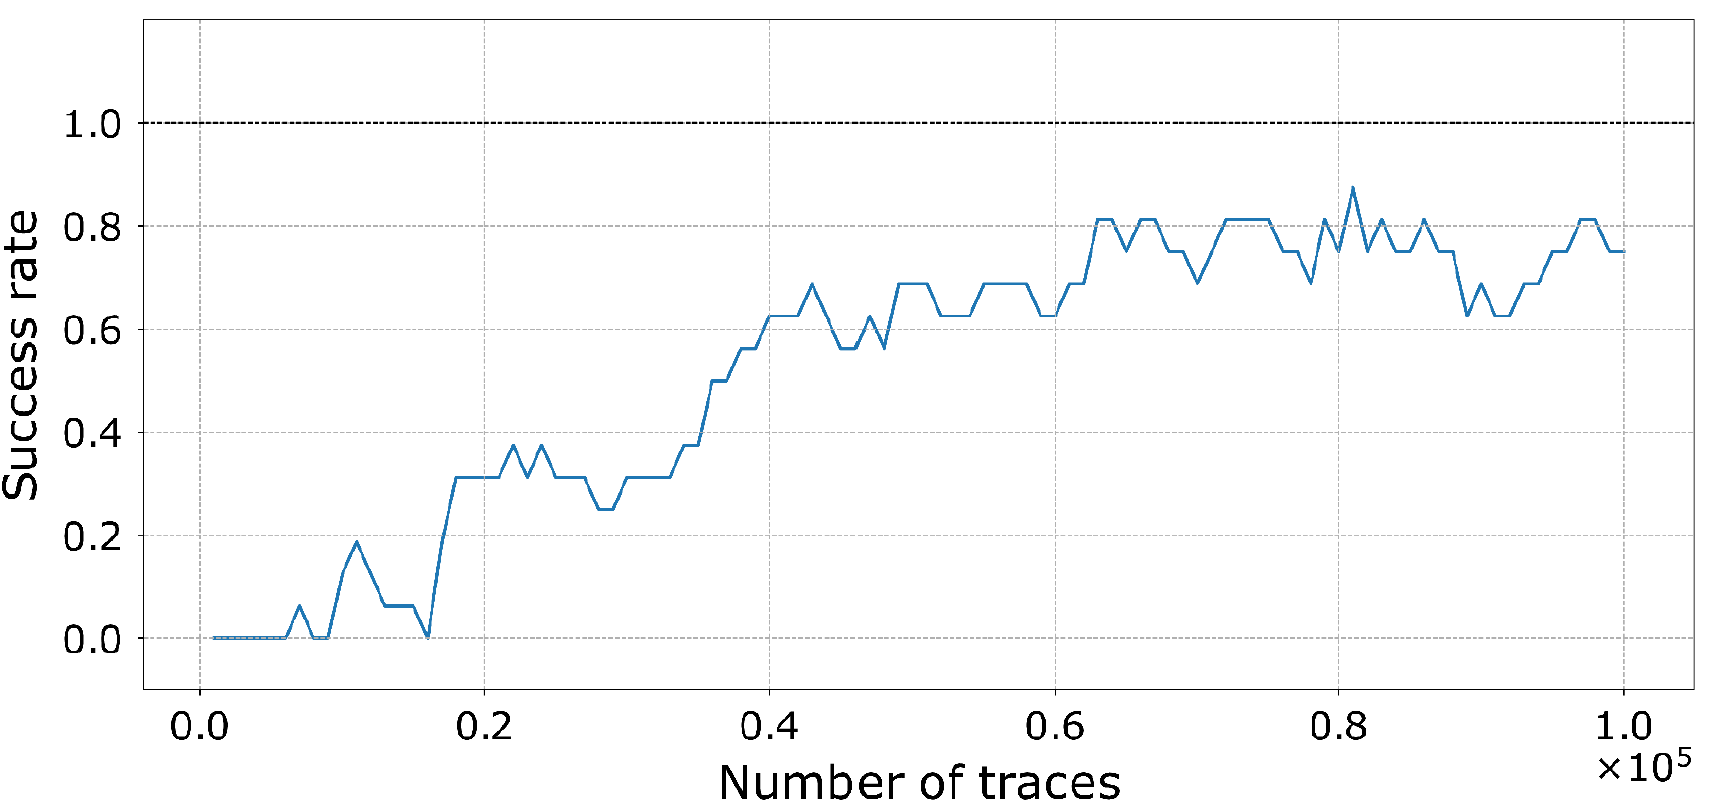
\includegraphics[width=0.8\textwidth]{metrics/Pictures/SR_plot_unprotected.png}
        \caption{for an unprotected AES using 16 parallel S-boxes, $SR$ (with 100,000 traces) is 1 only 80\% of the time}
    \end{figure}
\end{frame}
\begin{frame}
    \begin{block}{SR of Order $o$}
        The $SR$ metric can be extended to reflect cases where the correct key is ranked highly, but not necessarily 1st.
        
        $SR_i^o$ is 1 if the correct key $k_c$ is found within the top $o$ key guesses (i.e., $k_c \in [guess_1, \dots, guess_o]$ or $rank_{k_c} \le o$), otherwise 0.
        $$ SR_o^i = \begin{cases} 1, & \text{if } rank_{k_c} \le o \\ 0, & \text{otherwise} \end{cases} $$
        The overall $SR_o$ is:
        $$ SR_o = \frac{1}{p} \sum_{i=1}^{p} SR_o^i $$
        If $o=1$, this reverts to the original $SR$ definition.
    \end{block}
\end{frame}



\begin{frame}
    \frametitle{SR of Order $o$: Link to Attacker Effort}
        If an evaluator finds $SR^o=1$ for a key part, an attacker with an unknown key would need to verify at most $o$ candidates to find that key part after performing the attack.
        \newline
        \textit{Example:} If $SR^5=1$ for an AES byte, the attacker needs to check at most 5 candidates for that byte.
    
    \begin{block}{Full Key Enumeration Challenge}
        \begin{itemize}
            \item This key enumeration process must be repeated for all divide-and-conquer partitions of the full key.
            \item For example, if $SR^5=1$ for all 16 AES-128 key bytes, an attacker might need to verify up to $5^{16}$ full keys.
            \item This is a computationally challenging, heuristic task, and determining the appropriate value for $o$ is critical for assessing attacker capability.
        \end{itemize}
    \end{block}
\end{frame}


\begin{frame}
   
    \frametitle{Guessing Entropy (GE): Definition}
    
        To avoid the heuristic and potentially complex process of $SR$ of order $o$ for full key enumeration, Guessing Entropy (GE) offers a more flexible metric.
   
    
    \begin{block}{GE Formal Definition}
        Given a rank vector $[rank_0, rank_1, \dots, rank_{|K|-1}]$ and the correct key $k_c$, the rank of $k_c$ ($rank_{k_c}$) can be found and plotted against the number of traces.
        
        For a given experiment $i$, $GE_i$ is defined as:
        $$ GE_i = \log_2(rank_{k_c}) $$
        It is typically expressed in bits.
        
        The overall GE, averaged over $p$ experiments (where $k_c$ is ideally changed between experiments to ensure statistical stability), is:
        $$ GE = \frac{1}{p} \sum_{i=1}^{p} GE_i $$
    \end{block}
\end{frame}



\begin{frame}
    \frametitle{Guessing Entropy (GE): Interpretation and Example}

        The $rank_{k_c}$ and GE metrics represent the average remaining workload for an attacker after a side-channel attack.
        GE = 0 means the side-channel attack has eliminated all uncertainty about the secret key
            %\item For masked S-box implementations, GE stays substantially above 0 (about 8 bits even with 50,000 traces), showing that the attack leaves significant uncertainty and the device remains resistant.

    \begin{figure}
        \centering
        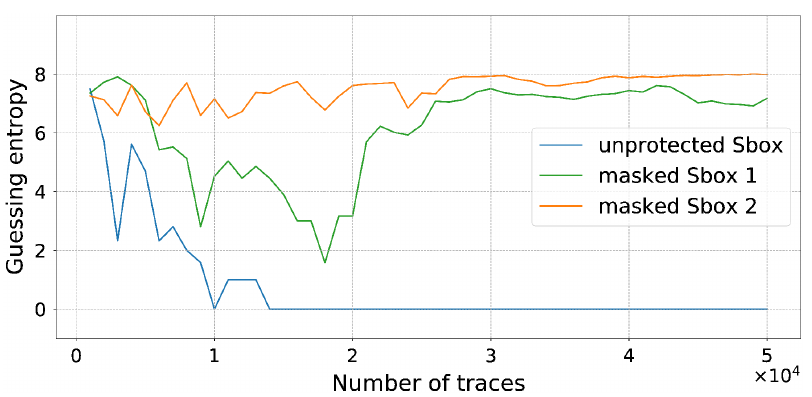
\includegraphics[width=0.75\textwidth]{metrics/Pictures/GE_plot.png}
        \caption{Guessing Entropy plot for three AES S-box implementations. GE drops to 0 for the unprotected S-box after roughly 15,000 traces; for masked S-boxes, GE remains high even with 50,000 traces.}
    \end{figure}
\end{frame}

%%%%REVIEW
\begin{frame}
    \frametitle{Limitations of SR and GE: Full Key Security}

    \begin{block}{Byte-wise Metrics Do Not Translate Directly}
        Both Success Rate (SR) and Guessing Entropy (GE) quantify attack effectiveness for individual key bytes (e.g., in AES). However, knowing the GE or SR for all bytes does \textbf{not} allow direct inference of the GE or SR for the full key.
    \end{block}

    \begin{itemize}
        \item The process of full key recovery requires \textbf{key rank estimation}, which is the known-key analog of key enumeration.
        \item Full key security assessment is more complex than simply combining values for each byte; detailed estimation methods are required.
    \end{itemize}
\end{frame}

\begin{frame}
    \frametitle{Limitations of SR and GE: No Projection of Effort}

    \begin{block}{Trace-Dependency Limits Security Forecast}
        SR and GE provide attack progress for a specific number of measured traces, but do not project future effort required for successful key recovery.
    \end{block}

    \begin{itemize}
        \item If SR or GE is close to random guessing (e.g., 1/256 for AES byte), one can only conclude the attack currently fails.
        \item The metrics do \textbf{not} indicate how many more traces would be needed to break the cipher, nor are they designed to forecast eventual success.
        \item GE is an expression of the remaining effort, but it is always derived from a specific number of measured traces.
    \end{itemize}

    \begin{block}{Towards Better Projections}
        This limitation led to the development of new metrics, which tie attack scores and success probabilities more rigorously to the number of traces.
    \end{block}
\end{frame}


\section{Correlation as a Metric}

\begin{frame}
    \frametitle{Correlation as a Metric: Motivation}

    \begin{block}{Why Correlation?}
        Most side-channel metrics (SR, GE, score, rank) require success in the attack, but provide little information on how many traces are theoretically needed for success, especially if the attack fails.
    \end{block}
    \begin{itemize}
        \item Correlation gives a way to estimate and project the effort needed to recover the key.
        \item It enables "security projections": estimating how many traces are needed for the correct key candidate to distinguish itself from others.
        \item This is particularly useful when the attack hasn't succeeded yet, allowing for predictive evaluation.
    \end{itemize}
\end{frame}

\begin{frame}
    \frametitle{Pearson Correlation and Trace Projection}

    \begin{block}{Pearson's Correlation in Side-Channel Analysis}
        In CPA (Correlation Power Analysis), Pearson's correlation coefficient $\rho$ is computed between:
        \begin{itemize}
            \item The observed leakage traces $l_1,l_2,\dots,l_n$
            \item The modeled leakages $g(f(x_i,k))$ for a given key candidate $k$
        \end{itemize}
        For the correct key $k_c$ denote this as $\rho_{k_c}$
    \end{block}
    $$ 
    \rho_{k_c} = \frac{
        \sum_{i=1}^n (l_i - \frac{1}{n}\sum_{j=1}^{n}l_j)
        (v_i - \frac{1}{n}\sum_{i=j}^{n}v_j)
     }{
        \sqrt{\sum_{i=1}^n (l_i - \frac{1}{n}\sum_{j=1}^{n}l_j)^2}
        \sqrt{\sum_{i=1}^n (v_i - \frac{1}{n}\sum_{j=1}^{n}v_j)^2}
     }
     $$
     \scriptsize where $v_i = g(f(x_i,k_c))$
\end{frame}


\begin{frame}
    \frametitle{When Does CPA Succeed?}

    \begin{block}{Success Criterion}
        A CPA attack succeeds if $|\rho_{k_c}|$ for the correct key is noticeably higher than the absolute correlations for all incorrect key candidates.
    \end{block}

    \begin{itemize}
        \item A common practical and theoretical assumption: for all incorrect keys, the expected correlation is close to zero.
        \item Thus, success is reduced to distinguishing $\rho_{k_c}$ from zero (not from other possible nonzero values).
    \end{itemize}

    \begin{block}{Why is this Useful?}
        If you know (or can estimate) the "true" value of $\rho_{k_c}$ post-attack, you can predict how many traces $n$ are required for reliable key recovery.
    \end{block}
\end{frame}

\begin{frame}
    \frametitle{Mangard's Shortcut: Projecting the Number of Traces}

    \begin{block}{Formula for the Projected Number of Traces}
        Given an estimate of $\rho_{k_c}$, the formula for predicting the number of traces needed for successful CPA key recovery is:
        \[
        n' = 3 + 8
        \left|
            \frac{z_{\alpha}}{ \ln \left( \frac{1+\rho_{k_c}}{1-\rho_{k_c}} \right) }
        \right|^2
        \]
        where:
        \begin{itemize}
            \item $z_\alpha$ is the z-score for desired type I error $\alpha$ (e.g., $z_{0.01}$ for $1\%$ error);
            \item $\rho_{k_c}$ is the estimated correlation for the correct key hypothesis.
        \end{itemize}
    \end{block}

    
            As $\rho_{k_c}$ decreases, the required number of traces grows quadratically. \newline
             Only the correct key's correlation needs to be estimated: no need to compute all candidate correlations.
      
\end{frame}

%%%%%%%%%%%%%%%%%%%%%%%%%%%%%%%%%%%%%%%%%%%%%%
%%%% POTREI AGGIUNGERE UNA SLIDE SU COME SCEGLIERE z_alpha (in particolare alpha che sta tra 10^-1 e 10^-4
%%%%%%%%%%%%%%%%%%%%%%%%%%%%%%%%%%%%%%%%%%%%%%%

% Correlation and SR

\begin{frame}
    \frametitle{Correlation and Success Rate (SR) Projection}

        Instead of just estimating the number of traces needed for a break, we can predict the \textbf{Success Rate (SR)} of a CPA attack for a given number of traces.
        
        This method, developed by Rivain, uses the statistical properties of correlation scores $\rho$ for all key candidates.
    
    \begin{block}{The Custom Correlation Coefficient}
        The analysis uses a slightly different correlation coefficient, $\ddot{\rho}_k$, for each key candidate $k \in K$:
        $$ \ddot{\rho}_k = \frac{1}{n} \sum_{i=1}^{n} g(f(x_i, k)) \cdot l_i $$
        The key candidate $k$ that maximizes this coefficient is chosen as the best guess by the CPA attack.
    \end{block}
\end{frame}

\begin{frame}
    \frametitle{Statistical Model of Correlation Scores}
    
    \begin{block}{A Multivariate Normal Distribution}
        The core insight is that the vector of all correlation scores, $\ddot{\rho} = [\ddot{\rho}_0, \ddot{\rho}_1, \dots, \ddot{\rho}_{|K|-1}]$, follows a \textbf{multivariate normal distribution}.
        
        This distribution is defined by a mean vector $\mu_{\ddot{\rho}}$ and a covariance matrix $\Sigma_{\ddot{\rho}}$.
    \end{block}
    
            The mean $\mu_k$ for each key candidate $k$ is:
        $$ \mu_k = \frac{1}{|X|} \sum_{x \in X} g(f(x, k) \cdot \hat{\mu}_v$$  \text{where } $v = f(x, k_c)$ 
        
        The covariance $\Sigma_{ij}$ between candidates $i$ and $j$ is:
       $$ \Sigma_{ij} = \frac{1}{n'|X|} \sum_{x \in X} g(f(x, i)) \cdot g(f(x, j)) \cdot \hat{\sigma}^2_v \quad \text{where } v = f(x, k_c) $$
        Here, $\hat{\mu}_v$ and $\hat{\sigma}^2_v$ are the mean and variance of the leakage for a given intermediate value $v$, estimated from experimental traces.
\end{frame}

\begin{frame}
    \frametitle{Projecting SR: The Methodology}
    
        The core of the method is to model the attack's outcome statistically.
        \begin{itemize}
            \item First, the leakage statistics ($\hat{\mu}_v$ and $\hat{\sigma}^2_v$) are estimated using an experimental set of traces.
            
            \item A \textbf{projected number of traces}, $n'$, is chosen. This value, which represents the strength of a hypothetical adversary, is used to define the covariance matrix $\Sigma_{\ddot{\rho}}$.
            
            \item Many random samples are then drawn from the resulting multivariate normal distribution, $\mathcal{N}(\mu_{\ddot{\rho}}, \Sigma_{\ddot{\rho}})$.
            
            \item Each sample vector represents a simulated attack outcome. It is sorted to find the rank of the correct key, $rank_{k_c}$.
            
            \item The \textbf{projected Success Rate (SR)} is the fraction of simulations where $rank_{k_c} = 1$. This can also be extended to find the projected $SR_o$.
        \end{itemize}
    
\end{frame}

\begin{frame}
    \frametitle{Limitations of Correlation-Based Projections}
    
    \begin{block}{ }
        \begin{itemize}
            \item  The projection formulas are based on \textbf{simplified statistical models}. The behavior of real hardware can deviate from these assumptions, due to electrical and electronic effects.
            
            \item \textbf{Estimation errors:} Imperfect statistical estimation of the correlation coefficient reduces the reliability of the results.
            
            \item \textbf{The purpose is Projection:} These are bounds designed to estimate effort when an attack has not yet succeeded, not to guarantee a break.
        \end{itemize}
    \end{block}
\end{frame}

\section{Information-Theoretic Metrics}

\subsection{Motivation for IT Metrics}

\begin{frame}
    \frametitle{Motivation for IT Metrics (1): The Rise of Multivariate Attacks}
    
     Side-channel analysis evolved beyond simple CPA to include powerful \textbf{multivariate attacks} like template attacks and linear regression analysis.
     \newline These advanced attacks can often recover a secret key with substantially fewer traces than their univariate counterparts.
   
    
    \begin{alertblock}{The Problem}
        Metrics like correlation and SNR are not easily extended to a multivariate setting. This created the need for new metrics that could fairly assess the risk posed by these stronger attacks.
    \end{alertblock}
\end{frame}

\begin{frame}
    \frametitle{Motivation for IT Metrics (2): Separating Device from Attacker}
    
  
    A key desire behind IT metrics was to distinguish between two separate concepts:
    \begin{enumerate}
        \item \textbf{The implementation:} a device and its countermeasures, which inherently leak information.
        \item \textbf{The attacker:} the specific methods and capabilities used to exploit that information.
    \end{enumerate}
  
    
        Instead of asking "Can my specific attack succeed?", IT metrics aim to answer:
        \vspace{0.3cm}
        
        \centering
        \textit{"How secure is this implementation against side-channel attacks in general?"}
        \vspace{0.3cm}
        
        This shifts focus away from attack-specific metrics (like SR and GE), allowing for more generic conclusions about the security of a device.
    
\end{frame}

\begin{frame}
    \frametitle{Information Theory Basics (1): Entropy}
    
    \begin{block}{Entropy H(X)}
        Entropy measures the average uncertainty of a random variable. Before an attack, we have an initial uncertainty about the secret key, $K$.
        
        For a discrete variable, it is defined as:
        $$ H(X) = - \sum_{x \in \mathcal{X}} \text{Pr}(X=x) \cdot \log_2(\text{Pr}(X=x)) $$
        The result is measured in \textbf{bits}.
    \end{block}
    
    \textbf{Example: An AES Key Byte} \newline
        If the secret key byte $K$ is uniformly random, there are 256 possibilities. The initial entropy is:
        $$ H(K) = \log_2(256) = 8 \text{ bits} $$
        This represents our total lack of knowledge before observing any leakage.
\end{frame}

\begin{frame}
    \frametitle{Information Theory Basics (2): Conditional Entropy}
    
    \begin{block}{Conditional Entropy $H(X|Y)$: Remaining Uncertainty}
        Conditional Entropy measures the uncertainty of a variable $X$ \textbf{given that you already know} the value of another variable $Y$.
        
        \vspace{0.3cm}
        
        \centering
        \textit{What is the remaining uncertainty of the key \textbf{K}, given that we have observed the leakage \textbf{L}?}
        
        \vspace{0.3cm}
        This is written as $\mathbf{H(K|L)}$. From a security perspective, we want this value to be as high as possible after an attack.
        $$H(X|Y)=-\sum_{x \in X, y \in Y}\text{Pr}(X=x,Y=y)\cdot\log(\text{Pr}(X=x|Y=y))$$
    \end{block}
\end{frame}

\begin{frame}
    \frametitle{Information Theory Basics (3): Continuous Variables}
    
  
        Since side-channel leakage is often an analog signal, we extend the concept of entropy to continuous random variables. 
        
        For a variable $X$ with a probability density function (PDF) Pr$(x)$, it is defined as:
        $$ H(X) = - \int_{X} \text{Pr}(X=x) \log_2( \text{Pr}(X=x)) \, dx $$
    
        The joint and conditional entropies for continuous variables `X` and `Y` are defined similarly:
        
        \textbf{Joint Entropy:}
        $$ H(X, Y) = - \iint_{X,Y} \text{Pr}(X=x, Y=y) \log_2 \text{Pr}(X=x, Y=y) \, dx dy $$
        
        \textbf{Conditional Entropy:}
        $$ H(X|Y) = - \iint_{X,Y} \text{Pr}(X=x, Y=y) \log_2 \text{Pr}(X=x|Y=y) \, dx dy $$
\end{frame}

\begin{frame}
    \frametitle{Information Theory Basics (4): Visual analogy}
    
    \begin{figure}
        \centering
        \includegraphics[width=0.8\textwidth]{placeholder.png} 
        \caption{Visualization of information-theoretic concepts with Venn diagrams.}
    \end{figure}
    
    %\begin{itemize}
    %    \item \textbf{H(K)} and \textbf{H(L)} represent the total uncertainty (entropy) of the key and the leakage, respectively.
    %    \item The \textbf{overlap} represents the \textbf{Mutual Information, I(K;L)}—the information they share.
    %    \item The part of H(K) that \textit{does not} overlap is the \textbf{Conditional Entropy, H(K|L)}—the uncertainty about the key that remains even after seeing the leakage.
    %\end{itemize}
\end{frame}

\subsection{Mutual Information}
\begin{frame}
    \frametitle{Mutual Information}
    
    \begin{block}{Definition}
        Mutual Information quantifies the amount of information that one variable ($Y$) provides about another ($X$). It is the \textbf{reduction in uncertainty} of $X$ after observing $Y$.
        
        It is fundamentally defined by the relationship between the entropies:
        $$ I(X;Y) = H(X) - H(X|Y) $$Theory
    \end{block}
    
    When applied to our problem, the formula becomes:
    $$ I(K;L) = H(K) - H(K|L) $$
    $$ \text{Information Leaked} = \text{Initial Uncertainty} - \text{Remaining Uncertainty} $$
    This metric, $I(K;L)$, represents the total amount of information (in bits) that the leakage $L$ reveals about the secret key $K$.
 
\end{frame}

\begin{frame}
    \frametitle{Mutual Information: Expanded Formulas}

    For discrete random variables $X$ and $Y$:
    $$
    I(X; Y) = \sum_{x \in X} \sum_{y \in Y} \Pr(X = x, Y = y) \cdot \log_2 \left( \frac{ \Pr(X = x, Y = y) }{ \Pr(X = x)\Pr(Y = y) } \right)
    $$


    For continuous random variables $X$ and $Y$ (using probability density functions):
    $$
    I(X; Y) = \int_{X} \int_{Y} \Pr(X = x, Y = y) \cdot \log_2 \left( \frac{ \Pr(X = x, Y = y) }{ \Pr(X = x)\Pr(Y = y) } \right) dx\,dy
    $$

    Mixed Case (Discrete $X$, Continuous $Y$)
        $$
        I(X; Y) = \sum_{x \in X} \int_{Y} \Pr(X = x, Y = y) \cdot \log_2 \left( \frac{ \Pr(X = x, Y = y) }{ \Pr(X = x)\Pr(Y = y) } \right) dy
        $$
\end{frame}


\begin{frame}
    \frametitle{Mutual Information: Visual Analogy}
    
    \begin{figure}
        \centering
        \includegraphics[width=0.8\textwidth]{placeholder.png} 
        \caption{Visualization of MI with Venn diagrams.}
    \end{figure}
    
    %\begin{itemize}
    %    \item \textbf{H(K)} and \textbf{H(L)} represent the total uncertainty (entropy) of the key and the leakage, respectively.
    %    \item The \textbf{overlap} represents the \textbf{Mutual Information, I(K;L)}—the information they share.
    %    \item The part of H(K) that \textit{does not} overlap is the \textbf{Conditional Entropy, H(K|L)}—the uncertainty about the key that remains even after seeing the leakage.
    %\end{itemize}
\end{frame}


\begin{frame}
    \frametitle{Applying MI to Side-Channels}
    
        We want a metric that can capture \textbf{multivariate leakages}. To do this, we move from thinking about a single leakage value $L$ to a leakage \textbf{vector} $\mathbf{L}$.
        
        \vspace{0.3cm}
        
        The goal is to use Mutual Information to quantify how many bits of information we can learn about the secret key $K$ by observing the multivariate side-channel leakage vector $\mathbf{L}$.
    
    \begin{alertblock}{}
        The definition remains the same, but the variables now have a specific meaning:
        $$ I(K;\textbf{L}) = H(K) - H(K|\textbf{L}) $$
        $$ \text{Information Leaked} = \text{Initial Uncertainty} - \text{Uncertainty after the Attack} $$
    \end{alertblock}
\end{frame}

\begin{frame}
    \frametitle{The MI Formula for Side-Channels}
    
        Applying the definitions of entropy and Bayes' rule, the MI between the key $K$ and the leakage $\mathbf{L}$ can be expressed as:
        
        $$ I(K;\mathbf{L}) = - \sum_{k \in K} \Pr(k)\log_2\Pr(k) + \sum_{k \in K} \Pr(k) \int_{\mathbf{l} \in \mathbb{R}^m} \Pr(\mathbf{l}|k) \log_2 \Pr(k|\mathbf{l}) \, d\mathbf{l} $$
    
    \begin{block}{What we need to compute}
        To solve this, an evaluator needs to know several quantities:
        \begin{itemize}
            \item The key probability, $\Pr(k)$.
            \item The conditional leakage probability, $\Pr(\mathbf{l}|k)$.
            \item The posterior key probability, $\Pr(k|\mathbf{l}) \rightarrow$ we can get rid of this thanks to Bayes
        \end{itemize}
    \end{block}
\end{frame}

\begin{frame}
    \frametitle{Simplifying the MI Formula}
    
        In the very common case where the secret key $K$ is \textbf{uniformly random}:
        \begin{itemize}
            \item The probability of any specific key is $\Pr(k) = 1 / |K|$.
            \item The initial entropy is simply $H(K) = \log_2 |K|$.
        \end{itemize}
    
    \begin{block}{Simplified Formula}
        Under this assumption, the MI formula simplifies significantly:
        $$ I(K;L) = \log_2|K| + \frac{1}{|K|} \sum_{k \in K} \int_{\mathbf{l} \in \mathbb{R}^m} \Pr(\mathbf{l}|k) \log_2  \frac{\Pr(\mathbf{l}|k)}{\sum_{k^* \in K} \Pr(\mathbf{l}|k^*)}  dl $$
    \end{block}
\end{frame}

\begin{frame}
    \frametitle{}
    
    \begin{alertblock}{}
        After all the simplification, the formula reveals that the \textbf{only remaining quantity} the evaluator needs to compute is:
        
  
        $$\Pr(\mathbf{l}|k)$$
        
   
        This term is the likelihood of observing a side-channel leakage vector $\mathbf{l}$, given a certain key $k$.
    \end{alertblock}
    
    \begin{block}{}
        The computation of this quantity is directly linked to \textbf{leakage profiling}, \textbf{leakage modeling} and parameter estimation.
    \end{block}
\end{frame}

\begin{frame}
    \frametitle{Modeling the Leakage to Compute $\Pr(\mathbf{l}|k)$}
    
        To find a value for $\Pr(\mathbf{l}|k)$, we create a statistical model of the leakage. A common approach, known as a \textbf{univariate template}, assumes the leakage for each key $k$ follows a \textbf{Normal (Gaussian) Distribution}.
        
        \begin{enumerate}
            \item This model is built using the workflow of a profiled attack, so the evaluator can use an open device to measure traces $[L_0^{prof},L_1^{prof},\dots,L_{255}^{prof}]$
            \item For normal distributions, leakage modeling is equivalent to estimating the mean ($\mu_k$) and standard deviation ($\sigma_k$) from the set of profiling traces.
            \item This gives us a list of leakage models $[\mathcal{N}(\mu_0, \sigma_0), \dots, \mathcal{N}(\mu_{255}, \sigma_{255})]$.
        \end{enumerate}
\end{frame}

\begin{frame}
    \frametitle{The Univariate Template}
    
    \begin{block}{}
        With the univariate template assumption, the probability of observing leakage $\mathbf{l}$ for a given key $k$ is given by the Gaussian probability density function:
        
        $$ \Pr(l|k) = \frac{1}{\sigma_k\sqrt{2\pi}} e^{ -\frac{1}{2} \left( \frac{l-\mu_k}{\sigma_k} \right)^2 } $$
    \end{block}
    
    By plugging this concrete model for $\Pr(l|k)$ into the simplified MI formula we saw earlier, we can now calculate a numerical value for the information leakage.
    $$I(K;L) = \log_2|K| + \frac{1}{|K|} \sum_{k \in K} \int_{-\infty}^{+\infty} \Pr(l|k) \log_2  \frac{\Pr(l|k)}{\sum_{k^* \in K} \Pr(l|k^*)}  dl $$
\end{frame}


%%% MAYBE aggiungere dettagli sull'implementazione Sbox masked
\begin{frame}
    \frametitle{Using MI to make projections on security}

    Mutual Information allows deriving security bounds, projecting the number of traces an attacker would need for key recovery.
    
    \textbf{Unprotected Implementation:}
    $$ \text{Number of traces} \ge \frac{H(K)}{I(L;K)} $$
    
    \textbf{d-th Order Masked Implementation:}
    $$ \text{Number of traces} \ge \frac{H(Y_i)}{I(L_i;Y_i) \cdot d} $$

    \begin{alertblock}{}
        These formulas are approximations that may overestimate an attacker's capabilities. However, because MI is inherently multivariate, they can provide a more fair security picture than correlation-based shortcuts.
    \end{alertblock}
\end{frame}

\begin{frame}
    \frametitle{Visualizing Security with MI}
    
    The value of MI directly reflects the security of a device, independent of any specific attacker's scores or ranks.
    
    \begin{itemize}
        \item \textbf{High MI} $\implies$ High information leakage $\implies$ Low security.
        \item \textbf{Low MI} $\implies$ Low information leakage $\implies$ High security.
    \end{itemize}

    \begin{figure}
        \centering
        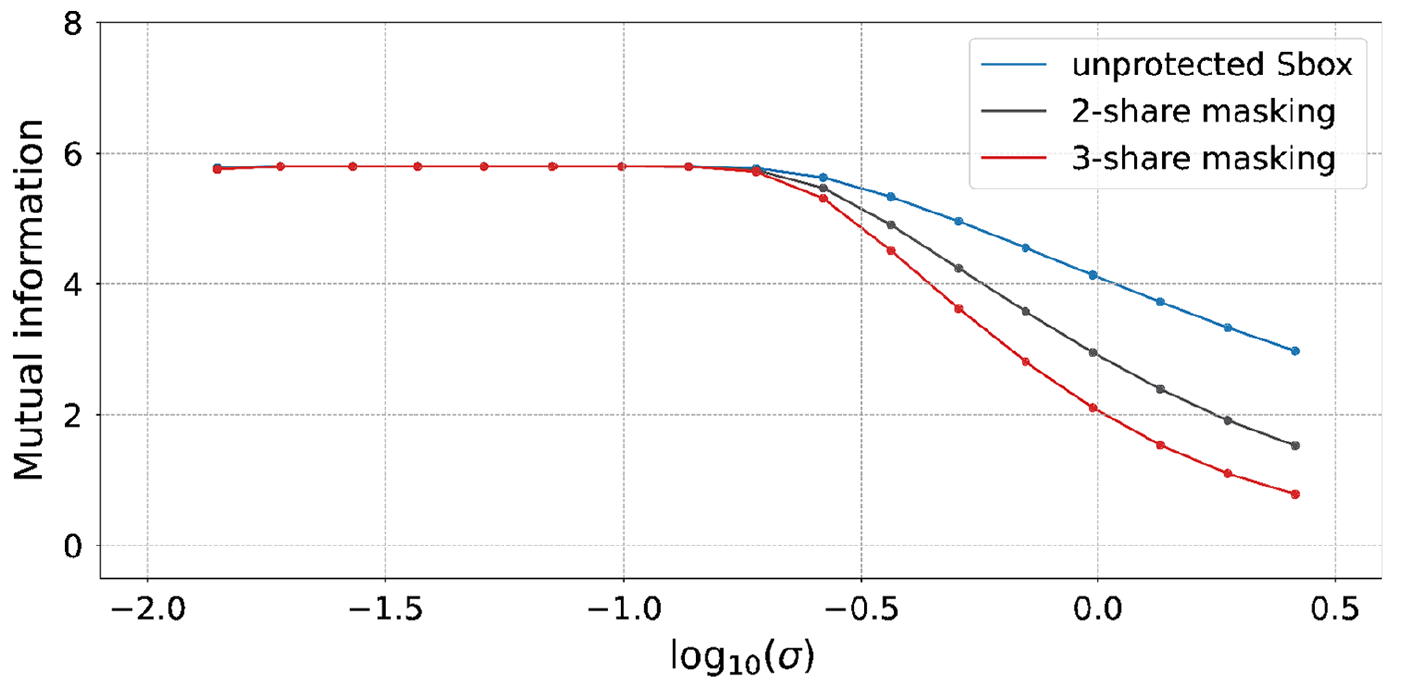
\includegraphics[width=0.8\textwidth]{metrics/Pictures/MI_masking.png}
        \caption{MI decreases as noise increases. Masking further amplifies this effect, showing its effectiveness as a countermeasure.}
    \end{figure}
\end{frame}




\subsection{Hypothetical Information}

\begin{frame}
    \frametitle{The Leakage Model: Two Scenarios}
    
    \begin{block}{Scenario 1: Theoretical Analysis (True Parameters)}
        Sometimes, an evaluator wants to test a countermeasure against a \textbf{theorized leakage model} without using experimental traces.
        \begin{itemize}
            \item \textbf{Example:} Assessing the security of a masking scheme against a perfect, non-linear leakage model.
            \item In this case, the model parameters (e.g., $\mu, \sigma$) are not estimated, but are \textbf{chosen} by the evaluator. These are considered the \textit{true parameters} for the theoretical model.
        \end{itemize}
    \end{block}
    
    \begin{block}{Scenario 2: Practical Evaluation (Estimated Parameters)}
        This is the case we discussed before. An evaluator uses a set of experimental profiling traces, $L_k^{prof}$, to \textbf{estimate} the model parameters ($\hat{\mu}, \hat{\sigma}$).
    \end{block}
\end{frame}

\begin{frame}
    \frametitle{Introducing Hypothetical Information (HI)}
    
    \begin{block}{Distinction in Terminology}
        To separate these two scenarios, the following terms are used:
        \begin{itemize}
            \item \textbf{Mutual Information (MI):} The metric calculated using \textbf{true parameters} from a theoretical leakage model. This achieves the goal of separating the implementation from the adversary.
            
            \item \textbf{Hypothetical Information (HI):} The metric calculated using \textbf{estimated parameters} ($\hat{\mu}, \hat{\sigma}$) from a real profiling dataset. This is what's computed in a practical evaluation.
        \end{itemize}
    \end{block}
    
    
\end{frame}

\begin{frame}
    \frametitle{The Pitfalls of Hypothetical Information (HI)}
    
        Unfortunately, an attacker's poor modeling is not fully reflected in the HI metric, which leads to two major types of errors.
    
    \begin{columns}[T] % Splits the frame into columns
        \begin{column}{0.5\textwidth}
            \textbf{1. Estimation Errors}
            \begin{itemize}
                \item Occur when the model is correct, but trained on \textbf{too few traces}.
                \item The resulting model is weak and may fail in a real attack.
                \item HI will still be positive and suggest that key recovery is possible, even when it is not.
            \end{itemize}
        \end{column}
        
        \begin{column}{0.5\textwidth}
            \textbf{2. Assumption Errors}
            \begin{itemize}
                \item Occur when the \textbf{chosen model is wrong} and does not reflect the device's actual leakage behavior.
                \item This can happen due to non-linear effects, measurement drift, or device differences.
                \item Even with infinite training data, the model is flawed. Yet, HI will likely be positive, suggesting an attack is possible when it's not.
            \end{itemize}
        \end{column}
    \end{columns}
\end{frame} 

\subsection{Perceived Information}

\begin{frame}
    \frametitle{The Fundamental Flaw of HI}
    
    The problem with HI is that it never \textbf{tests its own model against reality}.
        \begin{itemize}
            \item HI is calculated using only the profiling and modeling steps.
            \item It never considers a \textbf{test dataset} to see if the model's predictions actually match the device's real leakage.
            \item HI is "the amount of information that would be leaked from an implementation of which the leakages would be \textit{exactly predicted}" by the model.
        \end{itemize}
    
    
    \begin{alertblock}{}
    HI does not test its estimated model against the actual device leakage. \newline
        This gap is filled by a new metric that explicitly compares the model to reality: \textbf{Perceived Information (PI)}.
    \end{alertblock}
\end{frame}

\begin{frame}
    \frametitle{Cross Entropy}
    
    \begin{block}{}
        PI is built on the idea of \textbf{cross-entropy} $H_{p,q}(K|\mathbf{L})$. It measures the performance of a model distribution $q$ when it's used to describe a true distribution $p$.
        
        \begin{itemize}
            \item The \textbf{model distribution $q$} is our estimated model, $\hat{Pr}_{model}(\mathbf{l}|k)$, built from the profiling traces.
            \item The \textbf{true distribution $p$} is the actual leakage of the device, which we can only sample using a \textbf{ test data set}.
        \end{itemize}
    \end{block}
\end{frame}

\begin{frame}
    \frametitle{Introducing Perceived Information (PI)}
     \begin{block}{PI Definition}
        Perceived Information is defined as:
        $$ PI(\mathbf{L};K) = H(K) - H_{true, model}(K|\mathbf{L}) $$
        It subtracts the \textit{cross-entropy} between the true leakage and the model from the initial key entropy.
    \end{block}
    $$ PI(\mathbf{L};K) = (-\sum_{k \in K}\Pr(k)\log_2\Pr(k))-(-\sum_{k \in K,l \in L}\Pr_{true}(k|\mathbf{l})\log_2\hat{\Pr}_{model}(k|\mathbf{l})) $$
\end{frame}

\begin{frame}
    \frametitle{Computing PI}
   
        Assuming uniformly random keys and applying Bayes' rule, we get the general formula for Perceived Information:
        $$ PI(L;K) = H(K) + \sum_k \Pr(k) \sum_{l \in L_{k}^{test}} \Pr_{true}(l|k) \log_2 \left( \frac{\hat{\Pr}_{model}(l|k)}{\sum_{k^*} \hat{\Pr}_{model}(l|k^*)} \right) $$
    
    \begin{block}{}
        \begin{itemize}
            \item Computing $\hat{\Pr}_{model}(l|k)$ is identical to the computation of $\hat{\Pr(l|k)}$ in the HI metric
            
            \item To compute $\Pr_{true}(k|l)$  we distinguish between \textbf{simulated leakage} and \textbf{real traces}
        \end{itemize}
    \end{block}
\end{frame}

\begin{frame}
    \frametitle{Case 1: PI with Simulated Leakage}
    
    \begin{block}{Theoretical Scenario}
        In a theoretical analysis, the evaluator can \textbf{define} the true leakage distribution. For example, simulated traces can be generated with known characteristics (known noise level, ...).
        
        \begin{itemize}
            \item Here, $\Pr_{true}(l|k)$ is known because the evaluator created it.
            \item The PI metric then quantifies how well the estimated model, $\hat{\Pr}_{model}$, can capture this known, true distribution.
        \end{itemize}
    \end{block}
    
    \begin{alertblock}{}
        This scenario answers the question: \textit{"Is my training process good enough to learn this specific kind of leakage?"}
        
        A negative PI value in this case clearly indicates an \textbf{estimation error} (e.g., not enough training traces).
    \end{alertblock}
\end{frame}


\begin{frame}
    \frametitle{Visualizing Security with PI}
   \begin{figure}
        \centering
        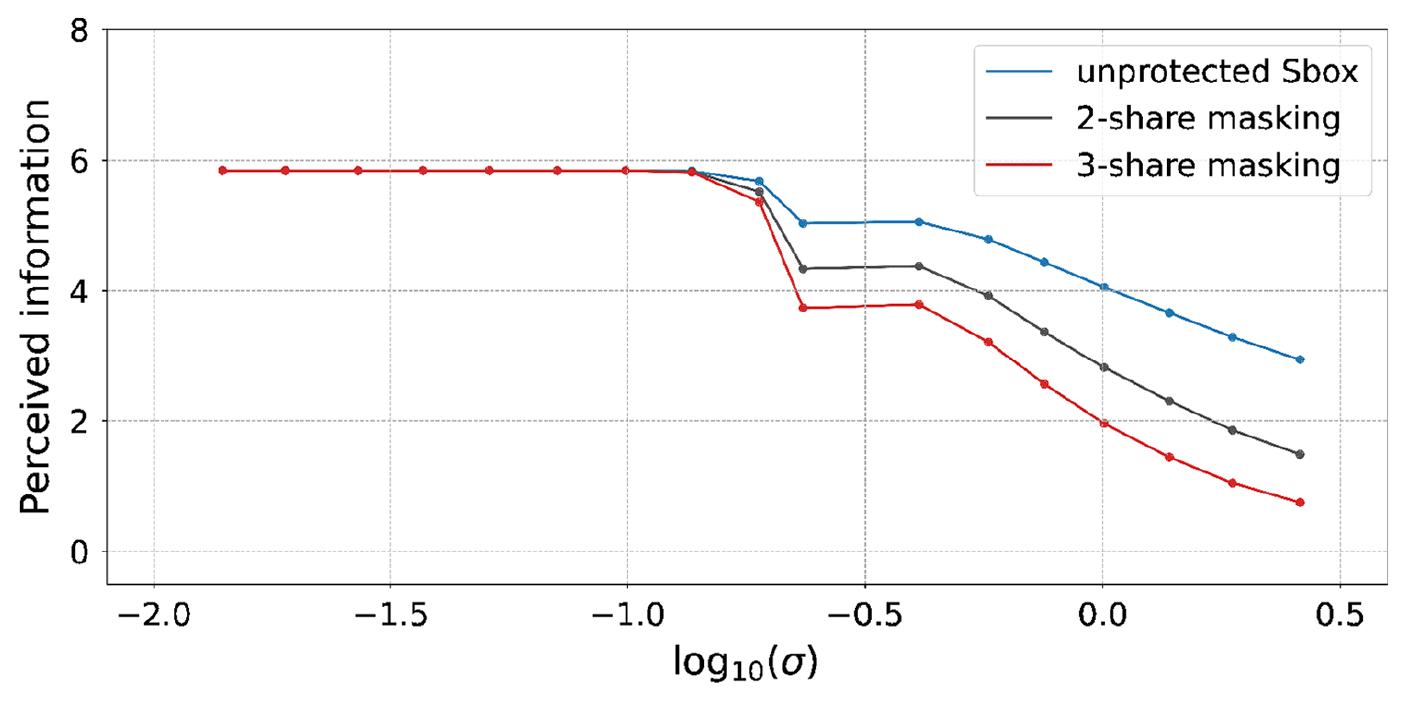
\includegraphics[width=0.8\textwidth]{metrics/Pictures/PI_masking.png}
        \caption{PI is positive and decreases as artificial white noise increases. The model training adequately captures the simulated leakage}
    \end{figure}
\end{frame}


\begin{frame}
    \frametitle{Case 2: PI with Real Traces}
    
    \begin{block}{Practical Scenario}
        In a practical evaluation of a real device, the true distribution is unknown. We can only \textbf{sample} it by collecting a \textbf{test dataset}, $L_k^{test}$.
        
        \begin{itemize}
            \item For each possible key $k$, we capture a new set of $n_k$ test traces.
            \item Sampling from the test set implies that the probability of observing any specific trace $l$ from that set is $\Pr_{true}(l|k) = 1/n_k$.
        \end{itemize}
    \end{block}
    
    \begin{alertblock}{The Practical PI Formula}
        This leads to the final, practical formula for PI:
        $$ PI(L;K) = H(K) + \sum_{k \in K} \frac{\Pr(k)}{n_k} \sum_{l \in L_k^{test}} \log_2 \left( \frac{\hat{\Pr}_{model}(l|k)}{\sum_{k^* \in K} \hat{\Pr}_{model}(l|k^*)} \right) $$
    \end{alertblock}
\end{frame}

\begin{frame}
    \frametitle{Comparison: Real and Simulated traces}
    
    \begin{block}{What Practical PI tells us}
        This metric directly answers the most important question for an evaluator:
        \vspace{0.3cm}
        
        \centering
        \textit{"Does my trained model capture the \textbf{actual device leakage} well enough to be useful?"}
    \end{block}
    
    \begin{block}{Detecting Errors}
        \begin{itemize}
            \item Unlike MI and HI, \textbf{PI can be negative}.
            \item A negative PI value proves that key recovery is not possible with the current model. It serves as a clear indicator of:
                \begin{itemize}
                    \item \textbf{Estimation errors} (not enough training data)
                    \item OR \textbf{Assumption errors} (the model is fundamentally wrong)
                \end{itemize}
        \end{itemize}
    \end{block}
\end{frame}

\begin{frame}
    \frametitle{Summary: The Hierarchy of IT Metrics}
    
        The three information-theoretic metrics are bound by the following important inequality:
        
        \vspace{1cm}
        \begin{itemize}
            
        \centering
        \huge
        $ PI \le MI \le HI $
        
        \end{itemize}{}
        \vspace{1cm}
    
    \begin{alertblock}{}
        The security bounds we saw earlier (for estimating the number of traces) can be computed with any of these metrics, but a calculation using PI is only meaningful \textbf{if the PI value is positive}.
    \end{alertblock}
\end{frame}

\subsection{Limitations of IT Metrics}

\begin{frame}
    \frametitle{Limitations of Information-Theoretic Metrics}
    
    \begin{enumerate}
        \item \textbf{Requires Generative Models:}
        The need for a probabilistic generative model (one that can describe the full leakage distribution) can exclude powerful discriminative models, like many neural network classifiers.
        
        \vspace{0.3cm}
        
        \item \textbf{Computational Hardness with High Dimensions:}
        IT metrics are naturally multivariate, but computing the required multi-dimensional integrals becomes extremely difficult as the number of leakage samples $m$ or masking shares $d$ increases.
        
        \vspace{0.3cm}
        
        \item \textbf{Difficulty with Horizontal Attacks:}
        Combining the leakage from multiple different intermediate values in the cipher (e.g., Sbox input and output) also dramatically increases the dimensionality and computational complexity.
    \end{enumerate}
    
    
        To resolve these issues evaluators often turn to techniques like Monte-Carlo integration, dimensionality reduction, or other approximations.
\end{frame}

\section{Key Enumeration and Rank Estimation}

\begin{frame}
    \frametitle{The Full Key Recovery Problem}

    The divide-and-conquer strategy gives us scores and ranks for each key \textbf{part} (e.g., each byte of an AES key).

    \begin{itemize}
        \item If the correct byte is Rank 1 for all 16 parts, recovering the full key is trivial.
        \item But what if some correct bytes have a lower rank? The attacker must test many combinations.
    \end{itemize}

    \begin{block}{The Central Question}
        How do we translate the security metrics for 16 independent 8-bit key parts into a single, meaningful security metric for the full 128-bit key?
    \end{block}

    This is solved by two related, but distinct, processes: \textbf{Key Enumeration} and \textbf{Rank Estimation}.
\end{frame}


\begin{frame}
    \frametitle{Key Enumeration: The Attacker's Approach}

    Key Enumeration is a practical process performed by an attacker in an \textbf{unknown-key} scenario.
    
    \begin{itemize}
        \item \textbf{Input:} The full set of scores for \textit{all} key candidates for \textit{all} key parts (e.g., 16 lists of 256 scores for AES-128).
        \item \textbf{Process:} Systematically construct and test full key candidates, starting with the most probable combinations derived from the scores.
        \item \textbf{Limit:} The process stops after a predefined number of attempts, $n_{en}$, which reflects the attacker's computational budget.
    \end{itemize}
    
    \begin{alertblock}{Binary Outcome}
        The result is a simple success or failure:
        \begin{itemize}
            \item \textbf{Success:} The correct full key is found within $n_{en}$ trials.
            \item \textbf{Failure:} The key is not found, and the attacker gives up.
        \end{itemize}
    \end{alertblock}
\end{frame}

\begin{frame}
    \frametitle{Key Enumeration}

    \textbf{Key Enumeration} is a practical process performed by an attacker in an \textbf{unknown-key} scenario.
    
    \begin{itemize}
        \item \textbf{Input:} The full set of scores for \textit{all} key candidates for \textit{all} key parts (e.g., 16 lists of 256 scores for AES-128).
        \item \textbf{Process:} Systematically construct and test full key candidates, starting with the most probable combinations derived from the scores.
        \item \textbf{Limit:} The process stops after a predefined number of attempts, $n_{en}$, which reflects the attacker's computational budget.
    \end{itemize}
\end{frame}
\begin{frame} {Key Enumeration}
    \begin{alertblock}{Measuring the Outcome}
        The outcome is a precise security level measured in bits of effort:
        \begin{itemize}
            \item \textbf{If the key is found in $n_e \le n_{en}$ trials}, the security of the device against this attack is exactly:
            $$ \text{security} = \log_2(n_e) \text{ bits} $$
            
            \item \textbf{If the key is not found within the limit}, the security is only known to be greater than the attacker's effort:
            $$ \text{security} > \log_2(n_{en}) \text{ bits} $$
        \end{itemize}
    \end{alertblock}
\end{frame}


\begin{frame}
    \frametitle{Rank Estimation}

    When key enumeration fails after $n_{en}$ attempts, the evaluator is left with a massive uncertainty gap. The true security could be anywhere from $n_{en}$ to $2^{128}$ (using AES-128 as our target).
    
    \begin{block}{Rank Estimation}
        To overcome this, the process of \textbf{Rank Estimation} was proposed. It is typically a \textbf{known-key analysis} that can:
        \begin{itemize}
            \item Quickly estimate the remaining brute-force effort for full key recovery.
            \item Achieve this without performing the costly process of listing all possible keys.
            \item Provide a precise security level even when the attack is not fully successful.
        \end{itemize}
    \end{block}

\end{frame}

\begin{frame}
    \frametitle{Rank Estimation: The Probabilistic Framework}

    To highlight the process, we use the \textbf{histogram-convolution-based algorithm} of Glowacz as our reference.

    \begin{block}{From Scores to Log-Probabilities}
        The process begins with the list of probabilities for each key candidate, which are converted to scores in the log domain:
        \[
            \text{score}_k^i = \log \Pr(k_i)
        \]
        where $i$ is the key part ($1, \dots, p$) and $k$ is the candidate ($0, \dots, m-1$).
        
        Assuming independence between key parts, the score for a full key is the sum of the scores of its parts:
        \[
             \Pr(\text{fullkey}) = \prod_{i=1}^{p}\Pr(k^i) \quad \iff \quad \log \Pr(\text{fullkey}) = \sum_{i=1}^{p} \log \Pr(k_i)
        \]
    \end{block}
\end{frame}

\begin{frame}
    \frametitle{Algorithm: Histogram-Based Rank Estimation}
    
    \begin{algorithm}[H]
    \begin{algorithmic}[] 
        \Statex \textbf{Input:} $\text{score}_k^i$, for $i=1, \dots, p$ and $k=0, \dots, m-1$
        \Statex \textbf{Output:} estimated rank, security (in bits)
        
        \For{$i = 1$ to $p$}
            \State $H^i \gets \text{hist}([\text{score}_0^i, \dots, \text{score}_{m-1}^i])$
        \EndFor
        
        \State $H \gets H_1$
        \For{$i = 2$ to $p$}
            \State $H \gets \text{conv}(H, H^i)$ 
        \EndFor
        
        \State $lp_c \gets \sum_{i=1}^{p} \log \Pr(k_c^i)$
        
        \State $\text{estimated\_rank} \approx \sum_{j=\text{bin}(lp_c)}^{\text{max\_bin}} H(j)$
        \State $\text{security} \gets \log_2(\text{estimated\_rank})$
    \end{algorithmic}
    \end{algorithm}
\end{frame}



\begin{frame}
    \frametitle{The Histogram-Based Method: Step-by-Step}

    The algorithm of Glowacz follows a three-step process to estimate the full key rank:

    \begin{enumerate}
        \item \textbf{Create Histograms:} For each of the $p$ key parts, compute a histogram of its $m$ scores (log-probabilities) using a fixed number of bins, $n_b$. This produces $p$ individual score distributions, $H_1, \dots, H_p$.
        
        \item \textbf{Convolve Histograms:} Iteratively convolve the $p$ histograms to produce a single final histogram, $H$. This final histogram represents the score distribution for the full key. This process introduces a small, unavoidable \textit{quantization error}.
        
        \item \textbf{Calculate the Rank:} Compute the total score of the correct key, $lp_c = \sum_{i=1}^{p} \text{score}_{k_c^i}$. Find which bin this score falls into, $\text{bin}(lp_c)$, and sum the counts of all bins corresponding to higher scores. This sum is the estimated rank.
    \end{enumerate}
\end{frame}


\begin{frame}
    \frametitle{Handling Quantization Error: Lower and Upper Bounds}
    
    The use of histograms introduces quantization errors. To account for this, the estimated rank is bounded to provide a reliable security range.
    
    \begin{block}{Rank Bounding Formulas}
        Given the final convoluted histogram $H$, the number of key parts $p$, and the correct key's score bin $\text{bin}(lp_c)$, the bounds are:
        
        \textbf{Lower Bound:}
        \[ \text{rank}_{\text{lower}} = \sum_{j=\text{bin}(lp_c)+p}^{\text{max\_bin}} H(j) \]
        
        \textbf{Upper Bound:}
        \[ \text{rank}_{\text{upper}} = \sum_{j=\text{bin}(lp_c)-p}^{\text{max\_bin}} H(j) \]
    \end{block}
    
    These bounds provide a tight and accurate estimation of the true key rank, as shown in experimental results on both simulated and real-world devices.
\end{frame}




%%% MAYBE ADD IMAGE FROM PAPER (pagina 29)
\begin{frame}
    \frametitle{A Tempting (But Wrong) Shortcut}
    
    It is tempting to estimate the full key rank by simply multiplying the ranks of the correct key parts (or, equivalently, summing their log-ranks).
    
    \begin{alertblock}{This is Incorrect and Misleading}
        This approach should be avoided for several reasons:
        \begin{itemize}
            \item It does not correspond to any valid key enumeration strategy an attacker would actually use.
            \item It falsely assumes the attacker has prior knowledge of the individual key part ranks, which they do not.
            \item As a result, it provides a \textbf{pessimistic lower bound} on the true rank, making the attack seem more effective than it is and underestimating the device's security.
        \end{itemize}
    \end{alertblock}
\end{frame}


\begin{frame}
    \frametitle{A Tempting (But Wrong) Shortcut}
    
    Consider a 4-bit key attacked as two 2-bit parts, $K_1$ and $K_2$, with the following probabilities:
    \begin{itemize}
        \item $\Pr(K_1) = [\texttt{00}:0.8, \textbf{01:0.1}, \texttt{10}:0.08, \texttt{11}:0.02]$
        \item $\Pr(K_2) = [\textbf{00:0.09}, \texttt{01}:0.5, \texttt{10}:0.01, \texttt{11}:0.3]$
    \end{itemize}
    The correct full key is $[\texttt{01}, \texttt{00}]$.
    
    \begin{columns}[T]
    \begin{column}{0.5\textwidth}
        \textbf{Shortcut Calculation:}
        \begin{itemize}
            \item The rank of $k_c^1=\texttt{01}$ is 2.
            \item The rank of $k_c^2=\texttt{00}$ is 3.
            \item Rank product = $2 \times 3 = 6$.
        \end{itemize}
    \end{column}
    \begin{column}{0.5\textwidth}
        \textbf{Optimal Enumeration:}
        \begin{itemize}
            \item An optimal enumeration strategy would list all 16 full keys by their true combined probability.
            \item The correct key $[\texttt{01},\texttt{00}]$ is found at position 9.
            \item The true rank is 9.
        \end{itemize}
    \end{column}
    \end{columns}
    
\end{frame}


\begin{frame}
    \frametitle{Limitations of Enumeration and Rank Estimation}

    \begin{alertblock}{}
        The optimality and soundness of these techniques depend on a critical condition: the attack scores must represent probabilities or log-probabilities.
    \end{alertblock}

    \begin{itemize}
        \item The underlying math assumes that scores for independent key parts can be combined via multiplication (for probabilities) or addition (for log-probabilities) to find the full key's probability.
        
        \item \textbf{Non-Bayesian scores}, such as raw correlation coefficients, have no such mathematically correct combination function.
        
        \item Applying simple heuristics like adding or multiplying these scores leads to inaccurate full key scores and a \textbf{suboptimal} enumeration or rank estimation.
    \end{itemize}

    \begin{block}{Practical Mitigation}
        Since Bayesian scores are not always available in practice, this limitation can be addressed with other heuristics, such as a \textbf{Bayesian extension}, which attempts to convert non-probabilistic scores into a usable format.
    \end{block}
\end{frame}



\section{Statistical Tests}

\begin{frame}
    \frametitle{Leakage Detection}

    Historically, side-channel research focused on creating new model-based and profiling attacks (e.g., DPA, CPA, Template Attacks).

    \vspace{2mm}
    \begin{block}{New Focus: Leakage Detection}
        Rather than developing new key-recovery attacks, the field is increasingly asking:
        \newline
        \begin{center}
            \textit{"Does a cryptographic device leak secret-dependent information at all?"}
        \end{center}
        The aim is to provide a reliable, attack-agnostic answer, supporting the validation of countermeasures.
    \end{block}
\end{frame}

\begin{frame}
    \frametitle{What is TVLA?}

    \textbf{Test Vector Leakage Assessment (TVLA)} is a standardized methodology for detecting side-channel leakage in a device without attempting full key recovery.

    \begin{itemize}
        \item TVLA analyzes whether a device leaks sensitive information when running known cryptographic algorithms.
        \item Instead of targeting unknown key bytes, TVLA tests whether any observable variable is correlated with any aspect of the secret.
        \item TVLA is especially useful for validating the \textbf{effectiveness of countermeasures}.
    \end{itemize}
\end{frame}

\begin{frame}
    \frametitle{The t-test in TVLA: The Goal and Hypothesis}

    The goal of the TVLA t-test is to formally certify a device's security status. The test uses two sets of traces captured with a fixed key:
    \begin{itemize}
        \item $\mathbf{L_r}$: A set of $n_r$ traces from \textbf{random} plaintexts.
        \item $\mathbf{L_f}$: A set of $n_f$ traces from a \textbf{fixed} plaintext.
    \end{itemize}
    
    \begin{block}{The Statistical Hypothesis}
        The abstract question "is the device secure?" is rephrased into a precise and testable hypothesis comparing the means ($\hat{\mu}$) of the two trace sets:
        
        \begin{itemize}
            \item \textbf{Null Hypothesis ($H_0$):} The means are equal. The device does not leak information detectable by this test.
            \[ H_0 : \hat{\mu}_r = \hat{\mu}_f \]
            \item \textbf{Alternative Hypothesis ($H_1$):} The means are different. The device exhibits leakage.
            \[ H_1 : \hat{\mu}_r \neq \hat{\mu}_f \]
        \end{itemize}
    \end{block}
\end{frame}

\begin{frame}
    \frametitle{Welch's t-test: The Calculation}

    To test the hypothesis, the evaluator uses the two-tailed Welch's t-test, which computes two key values for each time sample in the traces.

    \begin{block}{}
    \begin{itemize}
        \item \textbf{The t-statistic}, which measures the difference between the means relative to their variance:
        \[ t = \frac{ \hat{\mu}_r - \hat{\mu}_f }{ \sqrt{ \frac{\hat{\sigma}_r^2}{n_r} + \frac{\hat{\sigma}_f^2}{n_f} } } \]
        
        \item \textbf{The degrees of freedom (df)}, which defines the shape of the t-distribution:
        \[ df = \frac{ \left( \frac{\hat{\sigma}_r^2}{n_r} + \frac{\hat{\sigma}_f^2}{n_f} \right)^2 }{ \frac{\hat{\sigma}_r^4}{n_r^2(n_r-1)} + \frac{\hat{\sigma}_f^4}{n_f^2(n_f-1)} } \]
        where the sample means and variances are $\hat{\mu}_i = \frac{1}{n_i}\sum_{l \in L_i} l$ and $\hat{\sigma}_i^2 = \frac{1}{n_i-1}\sum_{l \in L_i} (l - \hat{\mu}_i)^2$.
    \end{itemize}
    \end{block}
\end{frame}

\begin{frame}
    \frametitle{Interpreting the Result: The Decision and Errors}

    The calculated t-statistic is an instance of a random variable $T$ that follows a Student's t-distribution. We use it to make a decision.

    \begin{alertblock}{The Decision Rule}
        The null hypothesis $H_0$ is \textbf{rejected} if the absolute value of the t-statistic exceeds a predefined threshold, $th$:
        \[ |t| > th \]
        A rejection means leakage has been detected.
    \end{alertblock}
\end{frame}

\begin{frame}
    \frametitle{Interpreting the Result: Errors}
    \begin{block}{Controlling for Errors}
        \begin{itemize}
            \item A \textbf{Type I Error} (false positive) occurs when we reject $H_0$ even though the device is secure.
            \item TVLA seeks to control this error probability at a significance level $\alpha$.
            \item This is the probability of detecting flaws when none exist:
            \[ \alpha = \Pr(\text{reject } H_0 | H_0 \text{ is true}) = 2\Pr(t > th) \]
            \item TVLA suggests a strict threshold of $\alpha = 10^{-5}$ to avoid this costly error.
        \end{itemize}
    \end{block}
\end{frame}

\begin{frame}
    \frametitle{Setting Thresholds and Understanding Errors}


    
    For the recommended $\alpha = 10^{-5}$ and with a high number of traces (degrees of freedom $>$ 1000), the threshold becomes a well-known value:
        \[ th \approx 4.5 \]


    \begin{block}{False Negatives}
        \begin{itemize}
            \item A \textbf{Type II Error} ($\beta$) is the failure to reject $H_0$ when it is false (i.e., declaring a device secure when it actually has flaws).
            \item The standard TVLA process focuses on controlling the Type I error ($\alpha$) and conducts independent tests on every sample point of the traces.
        \end{itemize}
    \end{block}
\end{frame}

\begin{frame}
    \frametitle{Using the t-test as a Metric}

    While formally a statistical test, the t-value is often used as a practical metric.
    
    \begin{itemize}
        \item Plotting the t-statistic over time provides a clear visual of leakage.
        \item As expected, unprotected implementations show high t-values, but flaws can also be detected in masked implementations, revealing practical imperfections.
    \end{itemize}
    
    \begin{alertblock}{A Heuristic for Further Analysis}
        High absolute t-values (or low p-values) indicate leaky time samples. This allows the evaluator to use the t-test as a guide for:
        \begin{itemize}
            \item Selecting specific points-of-interest for attacks.
            \item Performing more detailed leakage profiling on the most vulnerable parts of the operation.
        \end{itemize}
    \end{alertblock}
\end{frame}

\begin{frame}{}
    \begin{figure}
        \centering
        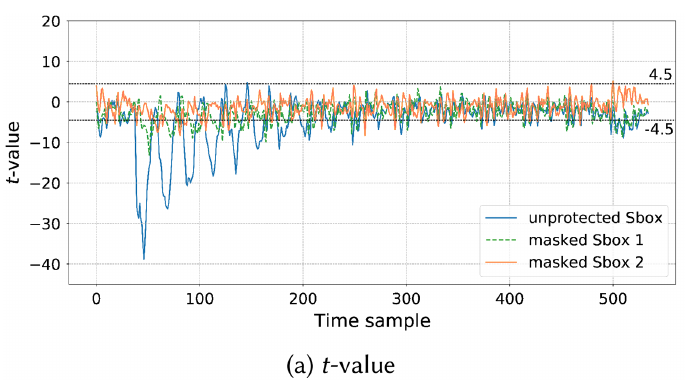
\includegraphics[width=0.65\linewidth]{metrics/Pictures/t_tet1.png}
        \label{fig:placeholder}
    \end{figure}
    \begin{figure}
        \centering
        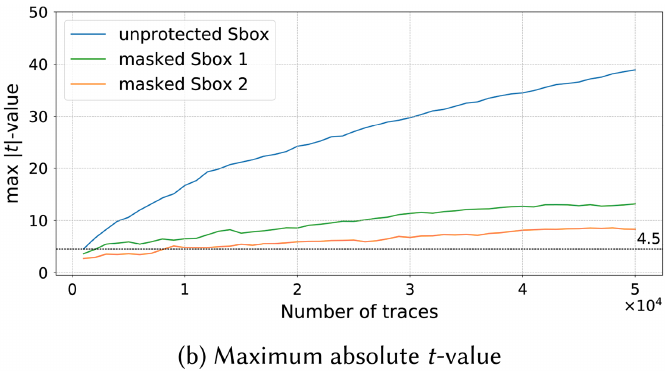
\includegraphics[width=0.65\linewidth]{metrics/Pictures/t_tet2.png}
        \label{fig:placeholder}
    \end{figure}
\end{frame}

\begin{frame}
    \frametitle{Trade-off for the experimenter }

    A key insight is that the t-value's significance depends more on the \textbf{parameters of the experiment} than on the results alone.
    
    \begin{block}{}
        The relationship between the number of traces ($n$), error rates ($\alpha, \beta$), signal variance ($\hat{\sigma}^2$), and the detectable effect size ($\delta$) is given by:
        \[ n = \frac{(\hat{\sigma}_r^2 + \hat{\sigma}_f^2)(z_{\alpha/2} + z_{\beta})^2}{\delta^2} \]
        Where $z_{\alpha/2}$ and $z_{\beta}$ are quantiles of the standard normal distribution.
    \end{block}
    
    This means any use of the t-value as a metric implicitly depends on all these parameters, which the evaluator must set in a meaningful way beforehand.
\end{frame}

\begin{frame}
    \frametitle{Variations and Best Practices for TVLA}
    
    The standard "random vs. fixed" test is powerful but has limitations and variations.
    
    \begin{itemize}
        \item \textbf{Limitation:} A negative result (no leak detected) from a single test is not conclusive, as it depends on the chosen fixed plaintext. \textbf{It is recommended to repeat the test with several different fixed inputs.}
        
        \item \textbf{Semi-fixed vs. random test:} A variation better suited for devices where the exact start/end of crypto operations is unclear.
        
        \item \textbf{Higher-order leakage:} The test can be adapted to assess masked implementations by first pre-processing traces to target higher-order statistical moments.
        
        \item \textbf{Specific tests:} If a non-specific test detects leakage, a specific test (requiring the key) can be used to confirm the finding with higher confidence by targeting a particular intermediate value.
    \end{itemize}
\end{frame}







\end{document}